\documentclass[11pt,letterpaper]{article}
\usepackage{cogsys}
\usepackage{cogsysapa}
\usepackage[utf8]{inputenc}
\usepackage[T1]{fontenc}
\usepackage{times}
\usepackage[pdftex]{graphicx} % use this when importing PDF files

 % First page headings for accepted submissions.
\cogsysheading{X}{20XX}{1-6}{X/20XX}{X/20XX}
 % First page headings for poster submissions.
%\cogsysposterheading{First}{2012}{1-18}

\ShortHeadings{Interactive Reasoning to Solve Knowledge Goals}
              {B.\ Bengfort and M.\ Cox}

\begin{document}

\title{Interactive Reasoning to Solve Knowledge Goals}

\author{Benjamin Bengfort}{bengfort@cs.umd.edu}
\address{Department of Computer Science, University of Maryland,
         College Park, MD 20742 USA}
\author{Michael T. Cox}{michael.cox@wright.edu}
\address{Wright State Research Institute,
         Beavercreek, OH 45431 USA}
\vskip 0.2in

\begin{abstract}
Knowledge goals represent the need to acquire information or data, to fill in gaps in the world knowledge of an entity or in the database of a system and are important parts of computational understanding systems. In this paper we present a taxonomy of knowledge goals broadly characterized as simple and complex. Simple knowledge goals can be solved through traditional information retrieval techniques or database queries. Complex knowledge goals require plans composed of simpler knowledge goals in order to answer how and why questions. We propose an interactive reasoning system that leverages a case-based methodology in order to solve knowledge goals.
\end{abstract}

\section{Introduction}

A \textit{knowledge goal} represents the need to acquire information or data to fill in gaps in a knowledge source \cite{ram_goal-based_1991}. For humans this is often takes the form of questions, and current research on question and answer systems focus on the semantic parsing of a natural language question to a structured database query or lambda calculus representation \cite{yahya_natural_2012,unger_template-based_2012,berant_semantic_2013}. These parsing approaches are making headway in the solution of simple knowledge goals, where the primary task is a retrieval from some structured knowledge base; especially goals that ask “who”, “what”, “when”, or “where”. This approach, however, cannot solve complex knowledge goals including aggregations – “how many countries have won three consecutive gold medals in the same sport?”, opinions – “what is the best restaurant in Boston?”, or explanations such as “why” or “how” questions.

Humans solve complex knowledge goals through \textit{investigation}, dividing harder questions into simpler sub-knowledge goals whose solutions are more easily obtained. When solving knowledge goals, humans also take into account context and approach new problems by leveraging techniques that have worked in the past. Investigation can be represented as a plan to solve the larger knowledge goal, and if the leaf nodes of knowledge acquisition plans are simple knowledge goals that can be solved via structured data retrieval, then a system can be said to compute complex knowledge goals through a planning process that involves the purposeful combination of simpler knowledge goals.

Goal driven natural language queries are therefore knowledge goals whose solution is a plan composed of simpler knowledge goals, the leaf nodes of which are computationally tractable tasks, e.g. database queries or document retrieval. Computational systems that automatically solve goal driven natural language queries must formulate plans which take into account the context of the goal and leverage a wide array of data sources to perform individual IR tasks. In this paper we will present the vision for an interactive computational system that makes use of case based reasoning in a mixed initiative environment to propose plans to the user then execute knowledge related tasks to arrive at the solution to complex knowledge goals. This type of system is adaptive and subject to goal changes, where the original knowledge goal is changed or refined slightly as a result of following some solution plan thus creating a \textit{goal trajectory}.

\section{Knowledge Goals}

\begin{figure}
	\centering
	    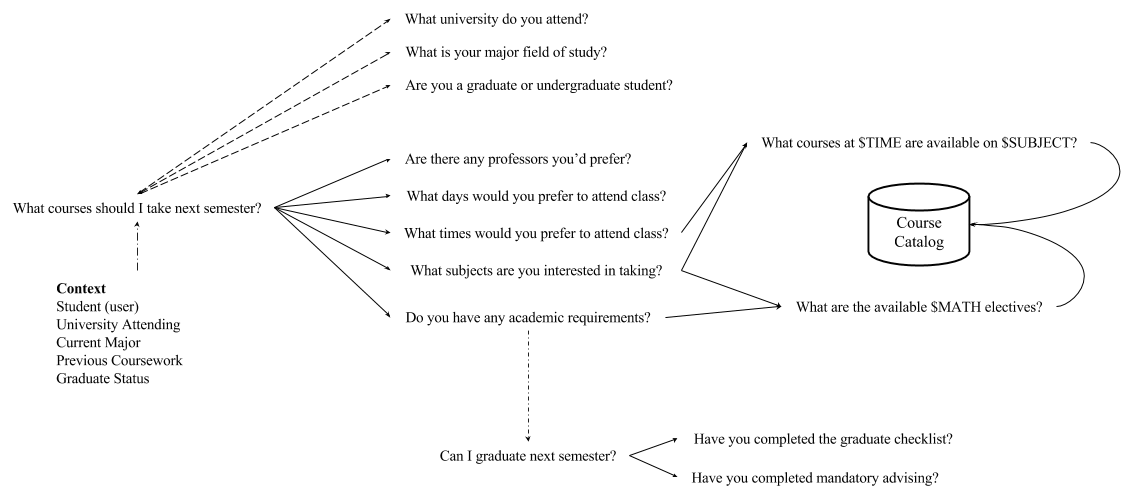
\includegraphics[width=\textwidth]{figures/simple_trajectory.png}
    \caption{\label{fig:simple_trajectory.png}A simple knowledge goal solution with trajectory change}
\end{figure}

Intelligent systems use knowledge goals to represent the need to acquire information and do so in a planful way \cite{ram_goal-based_1991}. Plans and knowledge goals are adaptable, subject to change as the system proceeds executing complex queries to discover knowledge and explanation \cite{munoz-avila_case-based_2008}. Goal trajectories can be influenced by other users in the system, either humans who are issuing similar queries and providing recommended goals through collaborative filtering \cite{hayes_case-based_2001} or via monitoring of automatic systems on new information or relevant data that has been added to the knowledge base. In either case, mixed-initiative goal changes can be seen as a planning problem that must be responsive to change \cite{cox_mixed-initiative_2007}.

Consider the example, “What courses should I take next semester?”. The task of this knowledge goal is to deliver a set of courses that the student will presumably register for. A question like this is routine, executed by the same users on a regular interval, and common enough that a large case-base of plans to solve the question is readily available. To solve this knowledge goal, the system might respond with sub-knowledge goals such as, “What days and times would you prefer?”, “Are there any subjects you're interested in?”, or “Do you have any academic requirements?”. Responses to these questions will lead to simple knowledge goals that can be queried against a course catalog, e.g. “What Economics courses are available on Monday and Wednesday?”.

Importantly, this knowledge goal is subject to change through the course of executing a planned solution. Changes in knowledge goals that lead to different solutions than originally presented play a vital role into understanding the creative aspects of the investigative process. In the above example, the goal may change from the acquisition of a list of courses to reasoning about whether or not graduation is possible next semester, or how soon graduation will occur.

In order to structure a successful interactive case-based reasoning system, the representation of a knowledge goal needs to be well defined, especially for purposes of retrieval and reuse. We propose a structured representation of a knowledge goal with three primary constructs: the \textit{concept}, the \textit{task}, and the \textit{context}. The concept relates the knowledge goal to all involved entities, either directly specified or implied and provides a domain to search upon. The task represents the purpose of the question, which also relates to the taxonomic characterization of the knowledge goal. Tasks determine the execution context of knowledge goal reasoning. Finally the user-specific context of the question provides input for refining plans or resolving ambiguities.

\section{Conclusion}

In this paper we have briefly presented a high-level taxonomy of knowledge goals: simple and complex and proposed a representation composed of the concept, task, and context to be used in a case-based interactive reasoning system. We've also shown that reasoning systems must be adaptive and responsive to change to mimic human investigative processes, leading to creativity by allowing for knowledge goal trajectories. For our upcoming research, we are currently building a system that allows the collection of knowledge goal cases, in order to pursue research on cognitive systems of investigation.

% \newpage

\vspace{-0.25in}

{\parindent -10pt\leftskip 10pt\noindent
\bibliographystyle{cogsysapa}
\bibliography{kgworkshop}

}

% Leave a blank line before the closing brace to ensure the final
% reference has the proper indentation.

\end{document}
